\renewcommand{\inputfile}{\version\ - Predrag edited 2014-10-28 cLvsLit}
% siminos/xiong/thesis/chapters/cLvsLit.tex
% $Author: xiong $ $Date: 2017-03-02 12:37:22 -0500 (Thu, 02 Mar 2017) $

% \section{\CLvs\ literature overview}
%        \label{sec:cLvsLit}

\newtheorem{floquet_theorem}{Flqouet Theorem}

\subsection{Floquet theorem and periodic orbits}

Linear ordinary differential equation with periodic
coefficients is an old topic. Solution of such type of
equations can be decomposed to a time-exponential part
and a bounded periodic part. The rigorous statement is given by
\begin{floquet_theorem}\cite{Floquet1883}
  \label{them:ft}
  If $\Phi(t)$ is a fundamental matrix solution of linear system
  $\dot{x} = A(t)x$ with periodic coefficients $A(t+T)=A(t)$,
  $T$ being the period, then $\Phi(t)$ can be decomposed as
  \[
    \Phi(t) = P(t)e^{tB} \quad \text{with} \quad P(t) = P(t+T)
    \,.
  \]
  Here $P(t)$ is called monodromy matrix, and $B$ is a constant
  matrix. Eigenvalues of $B$ are called Floquet exponents. The
  eigenvectors are called Floquet vectors.
\end{floquet_theorem}
The proof of this theorem is very simple. First, it is easy to
see that if $\Phi(t)$ is solution matrix, so is $\Phi(t+T)$.
Their relation is given by $\Phi(t+T)=\Phi(t)C(t, T)$, where
$C(t, T) = \Phi^{-1}(t)\Phi(t+T)$. Second, $C(t, T)$ is independent
of time which can be shown by taking time derivative
at both sides of $\Phi(t)C(t, T) = \Phi(t+T)$, so matrix $C(T)$
is only parametrized by the period. Furthermore,
$C(aT) = \prod_{k=0}^{a-1}\left(\Phi^{-1}(t+kT)\Phi(t+kT+T)\right) = C(T)^a$;
thus $C(T)$ has form $e^{TB}$, where $B$ is a constant matrix.
So $\Phi(t+T)=\Phi(t)e^{TB}$. Last,
If we define a new matrix $P(t) = \Phi(t)e^{-tB}$, then
$P(t+T) = \Phi(t+T)e^{-TB-tB} = \Phi(t)e^{-tB} = P(t)$. In this way,
we decompose the fundamental matrix solution into a periodic part
$P(t)$
and a time exponential part $e^{tB}$,
even though we do not know the explicit
form of $P(t)$.

Floquet theorem in condense matter physics is under another name
: \textbf{Bloch theorem}, which states that wave function in a periodic
potential can be written as
$\psi(\vec{r}) = e^{i\vec{k}\cdot\vec{r}}u(\vec{r})$.
Here $u(\vec{r})$ is a periodic function with the same potential period.
Eigenstates are classified into different bands by different profiles of
$u(\vec{r})$.

For our interest, dynamics in the tangent space
in nonlinear dynamical system is governed by $\dot{J} = A(x)J$.
Especially, for periodic orbits, $A(x)$ is periodic, and if we start
with $J(t_0) = I$, then Jacobian corresponding to one period $J_p$ is
just the exponential part $e^{TB}$ in theorem \ref{them:ft}.
This is the theoretical basis of periodic eigendecomposition algorithm,
which tries to calculate the eigenvalues and eigenvectors of $J_p$.
On the other hand, the periodic part $P(t)$ in theorem \ref{them:ft}
evolves Floquet vectors along the periodic orbit, and return to
the initial values after one period. This information is revealed
in the reordering stage of periodic eigendecomposition algorithm.


\newpage

\noindent{\bf Predrag, to us:} Here are the relevant articles.

\begin{description}
\item[Characterizing dynamics with covariant Lyapunov
              vectors,] by
Ginelli, Poggi, Turchi, Chat\'{e}, Livi and Politi\rf{ginelli-2007-99}
is the main reference on the
`covariant Lyapunov vectors.' They describe the QR algorithm for
computing Gram-Schmidt vectors (GSV) and recovering
the covariant Lyapunov vectors (CLV) from them.
They show, using covariant Lyapunov vectors, that
  the chaotic solutions of four spatially-coupled maps,
(a) chaotic tent maps,
(b) chaotic symplectic maps,
(c) continuous time rotator model, and
(d) Fermi-Pasta-Ulam chain
  evolve within a manifold spanned by a finite number
  of {\entangled} modes.

\item[Hyperbolicity and the effective dimension] of
    spatially-extended dissipative
    systems, by Yang, Takeuchi, Ginelli, Chat\'{e}
    and Radons\rf{YaTaGiChRa08},
 is a demonstration of what we
  have observed numerically, that a finite number of Fourier modes
  captures most of the dynamics of KS, and most relevant to our research.
 They show, using {\cLvs}, that
  the chaotic solutions of two spatially extended dissipative
  systems, \KS\ and complex Landau-Ginzburg,
  evolve within a manifold spanned by a finite number
  of {\entangled} modes hyperbolically isolated from a set of
  residual degrees of freedom, themselves individually
  isolated from each other. The number grows linearly with
  $L$ and is twice as large as the Kaplan-Yorke dimension estimates.
  The results imply that a
  faithful numerical integration of dissipative
  partial differential equations needs to incorporate at
  least all {\entangled} modes and that increasing the resolution
  beyond that
  merely increases the number of isolated modes.

\item[\bf 2009-09-16 Lyapunov vectors, illustrated.]
In order to spare you from reading the source literature, I'm including here
those figures from Yang \etal\rf{YaTaGiChRa08} that I find most striking.
The main advance of using Lyapunov vectors instead of eigenvalues alone
is that the approximate orthogonality of the `isolated' ones provides a clear
threshold between the `{\entangled}' and the rest.

You might be unimpressed by the KS example, as the $-k^4$ hyper-diffusion
term kills all higher Fourier modes very effectively. For that reason the
complex Ginzburg-Landau equation, \reffig{fig:lyapSpecCLG}
is very persuasive; the nonlinearity is
of $u(x)^3$ variety (instead of $u \partial u$ of Navier-Stokes and
KS), but there is only a $-k^2$ diffusive term, and nevertheless there
is a clear threshold for the `isolated' Lyapunov vectors. Furthermore,
the system exhibits left and right traveling waves, which is more like
fluids than the rigid wave patterns of KS.
    \PC{2014-10-25 figure out why \reffig{fig:lyapSpecCLG} graphs are
    missing?}

\begin{figure}
 (a)~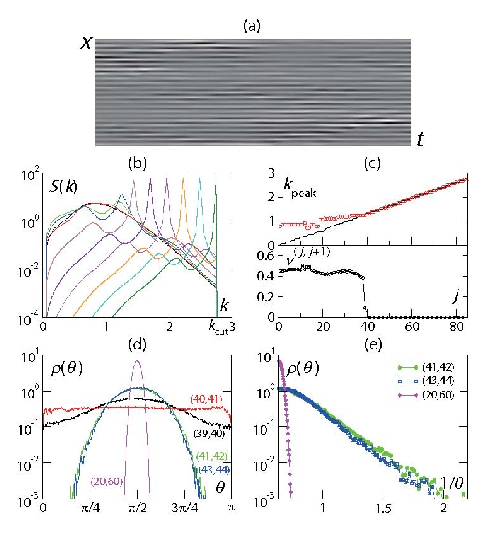
\includegraphics[width=0.45\textwidth]{YaTaGiChRa08fig2}
 (b)~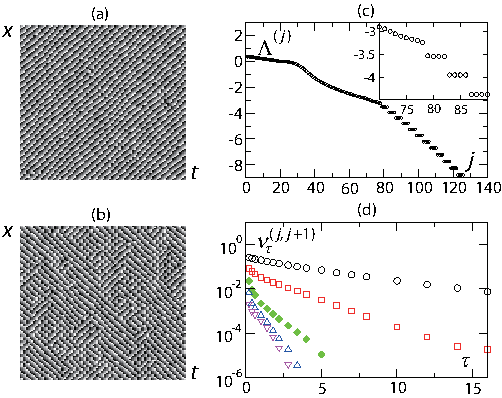
\includegraphics[width=0.45\textwidth]{YaTaGiChRa08fig3}
\caption{
(left panel)
Fig.~2 of Yang \etal\rf{YaTaGiChRa08}:
Properties of {\cLvs} for the KS system
($L = 96$, $k_{\rm cut} = 42 \cdot 2\pi/L$, and PBC).
(a) Spatiotemporal plot of a typical vector in the isolated region
($j=46$, total time $100$).
(b) Spatial power spectra of vectors of indices
$j = 1$, $16$, $32$, $38$, $44$, $52$, $60$, $68$, $76$, $84$
(from left to right in peak position).
(c) Top panel: peak wavenumber in the power spectra (red circles)
and $k = [j/2] \cdot 2\pi/L$ (black line).
Bottom panel: DOS violation fraction $\nu^{(j,j+1)}_\tau$ for pairs of
neighboring vectors (pairs within the same step are omitted).
(d) Angle distributions between pairs of vectors.
(e) Same as (d) but with a different abscissa.
(right panel)
Fig.~3 of Yang \etal\rf{YaTaGiChRa08}:
Complex Ginzburg-Landau equation in the amplitude turbulence regime
($L = 64$, $k_{\rm cut} = 31 \cdot 2\pi/L$, and PBC).
(a,b) Spatiotemporal plots of the phase component of a typical vector $j = 91$ in the isolated region
(same trajectory, but at two distant periods of time, during a total time of $20$ for each plot).
(c) Lyapunov spectrum; inset: close-up around threshold.
(d) Time fraction $\nu^{(j,j+1)}_\tau$ of DOS violation, as a function of $\tau$
($j=78$, 82, 86, 90, 94, from top to bottom).
}
\label{fig:lyapSpecCLG}
\end{figure}



\item[Lyapunov analysis and the collective dynamics]
of large chaotic systems\rf{TaGiCh09}:
Not as directly relevant to us as \refref{YaTaGiChRa08}.
They show, using globally-coupled (a) limit-cycle oscillators
(b) noisy logistic maps, that the collective dynamics
of large chaotic systems is encoded in their Lyapunov spectra:
most modes are typically localized on a few degrees of freedom,
but some are delocalized, acting collectively on the trajectory.
For globally-coupled maps, they show moreover a quantitative
correspondence between the collective modes and some of the
so-called Perron-Frobenius dynamics.


\item[An efficient method for recovering Lyapunov vectors] from
singular vectors\rf{WoSa07}:
\\
{\bf Predrag 2009-10-15} Wolfe
and Samelson seem to be the most important article to
understand. If Ginelli \etal\rf{ginelli-2007-99} say the key
thing (how to compute covariant eigenvectors, actually) they
hide it well.
Wolfe and Samelson say: `` Standard techniques for computing
Lyapunov vectors produce results which are norm-dependent and
lack invariance under the linearized flow. An efficient,
norm-independent method for constructing the $n$ most rapidly
growing Lyapunov vectors from $n\!-\!1$ leading forward and  $n$
leading backward asymptotic singular vectors is proposed. The
Lyapunov vectors so constructed are invariant under the
linearized flow in the sense that, once computed at one time,
they are defined, in principle, for all time through the
tangent linear propagator.
	\PC{remember `the tangent linear propagator'}		\inCB
An analogous method allows the
construction of the $n$ most rapidly decaying Lyapunov vectors
from $n$ decaying forward and $n\!-\!1$ decaying backward singular
vectors. ''

\HREF{http://www.mpipks-dresden.mpg.de/~ecodyc10/Contributions/Samelson.pdf}
{This talk} might be a quick introduction to the main points of their
paper.

\item[From synchronization to Lyapunov exponents and
              back]\rf{PoGiYaMa06}:
The early paper in this series.
In the first part they discuss a general approach to determine
Lyapunov exponents from ensemble- rather than time-averages.
The approach passes through the identification of locally
stable and unstable manifolds (the Lyapunov vectors), thereby
revealing an analogy with generalized synchronization. The
method is then applied to a periodically forced chaotic
oscillator. The
analytical calculations are carried out for a model, the
generalized special flow, that they construct as a simplified
version of the periodically forced R\"ossler oscillator.

\item[Structure of characteristic {L}yapunov vectors]
in spatiotemporal chaos\rf{PaSzLoRo09}:
They study Lyapunov vectors (LVs) corresponding to
the largest Lyapunov exponents in systems with spatiotemporal
chaos. They focus on characteristic LVs and compare the results
with backward LVs obtained via successive Gram-Schmidt
orthonormalizations. Systems of a very different nature such
as coupled-map lattices and the (continuous-time) Lorenz `96
model exhibit the same features in quantitative and
qualitative terms. They propose a minimal
stochastic model that reproduces the results for chaotic
systems.

\item[The predictability of a flow] which possesses
                many scales of motion\rf{lorenz69},
AKA Lorenz 1969 36-variable method is beloved by weathermen:
we might consider using it as a test of our higher\dmn\
visualizations.

\item[Periodic orbits, Lyapunov vectors, and singular
    vectors] in the Lorenz system\rf{TrePan98}:
{\bf Predrag 2009-10-15} Trevisan and Pancotti apparently
need to be cited for the observation that {\cLvs}
reduce to Floquet eigenvectors in the particular case of a
{\po} (seems so obvious it is in ChaosBook without
attribution, and Ruelle and Eckmann\rf{eckerg} surely say
that... Wolfe and Samelson\rf{WoSa07} are inspired by this
article, but seem to go beyond it. Trevisan and Pancotti say
``
A {\po} analysis in the Lorenz system
and the study of the properties of the associated tangent
linear equations are performed.
	\PC{noted `the associated tangent linear equations' in
        ChaosBook}		                                \inCB
A set of vectors are found
that satisfy the Oseledec (1968) theorem\rf{lyaos} and reduce to
Floquet eigenvectors in the particular case of a periodic
orbit. These vectors, called Lyapunov vectors, can be
considered the generalization to aperiodic orbits of the
normal modes of the instability problem and are not
necessarily mutually orthogonal. The relation between
singular vectors and Lyapunov vectors is clarified. The
mechanism responsible for super-Lyapunov growth is shown to
be related to the nonorthogonality of Lyapunov vectors. The
leading Lyapunov vectors, as defined here, as well as the
asymptotic final singular vectors, are tangent to the
attractor, while the leading initial singular vectors, in
general, point away from it. Perturbations that are on the
attractor can be found in the subspace of the leading
Lyapunov vectors.
    ''

\item[On the concept of stationary {L}yapunov basis] by Ershov
and Potapov\rf{ErshPot98}, available on
\HREF{http://www.math.ualberta.ca/~apotapov/Publications.htm}
{http://www.math.ualberta.ca/$\sim$apotapov}. They establish
existence of `stationary {L}yapunov basis'					\inCB
$\{\jEigvec[1],\cdots,\jEigvec[d]\}$ (called elsewhere `{\cLvs}') such that the Lyapunov
exponents are given by										
\beq
    \eigExp[j] = \lim_{N \to \infty} \frac{1}{N}
         \sum_{n=1}^{N} \ln
    |\jEigvecT[j](\ssp_n) \jMps(\ssp_n) \jEigvec[j](\ssp_n)|
\ee{ErshPotMap}
for a map, and
\beq
    \eigExp[j] = \lim_{T \to \infty} \frac{1}{T}
         \int_0^{T}dt
    \jEigvecT[j](\ssp(t)) \Mvar(\ssp(t)) \jEigvec[j](\ssp(t))
\ee{ErshPotFlow}
for a flow.
	\PC{looks wrong, needs exponentiation, time ordering?}
They say Goldhirsch, Sulem and Orszag\rf{GoSuOr87}
did the same thing, but for ODEs rather than maps.
Skokos also pointed me to Goldhirsch \etal. We should also
talk with Dieci\rf{DiEl08,DiRuVl97,DiVl02},
as he is at GaTech and seems to have
worked on closely related problem, the singular value decomposition
(SVD) to approximate Lyapunov spectra.

\item[2010-07-01 Predrag] reading
Goldhirsch, Sulem and Orszag\rf{GoSuOr87}:

The original Lyapunov article is \refref{Lyap1892},
but the key reference is 1968 Oseledec\rf{lyaos} -
they also cite various Farmer etc articles we do not seem to
cite any longer.

They refer to the \stabmat\ as `the Hessenberg matrix.'
    \PC{cite in ChaosBook stability.tex, and the
    equation of variations as `stability equations.'
    }										\inCB
Oseledec refers to an {\em orthonormal} set of vectors such
that their rate of growth defines Lyapunov exponents.

A \emph{stable limit cycle} has one zero exponent   \inCB
(perturbation tangent to the
cycle) and all other exponents negative.
Every attractor has at least one such zero eigenvalue.

Lyapunov exponents \emph{are not related} to the (stability)
Floquet exponents, so they discuss the relation between
`Lyapunov' and `stability' exponents.
\PC{cite in ChaosBook stability.tex}						\inCB

\item[2011-07-01 Predrag]
Greene and Kim\rf{GreeKim87} have a nice discussion of singular
values vs. \jacobianM\ eigenvalues. They believe that ``singular values,
rather than eigenvalues, are the appropriate quantities to consider
when studying chaotic systems.'' Their Fig.~3 illustrates various semiaxes
of the ellipsoid in the case of Lorenz; for me it is a motivation {\em not}
to use singular values.
\PC{cite in ChaosBook stability.tex}						\inCB

\item[2011-07-16 Predrag]
{\em Stabilization of long-period periodic orbits
    using time-delayed feedback control} by Claire
    Postlethwaite\rf{Postle09}
is perhaps of interest. She says: ``
The Pyragas method of feedback control has attracted much interest as a
method of stabilizing unstable periodic orbits in a number of situations.
We show that a time-delayed feedback control similar to the Pyragas
method can be used to stabilize periodic orbits with arbitrarily large
period, specifically those resulting from a resonant bifurcation of a
heteroclinic cycle. Our analysis reduces the infinite\dmn\
delay-equation governing the system with feedback to a three\dmn\
map, by making certain assumptions about the form of the solutions. The
stability of a fixed point in this map corresponds to the stability of
the periodic orbit in the flow, and can be computed analytically. We
compare the analytic results to a numerical example and find very good
agreement.
''






\item[Computing {L}yapunov spectra] with continuous
         {Gram-Schmidt} orthonormalization.
Christiansen and Rugh\rf{ChRu97},
present a
  continuous method for computing the Lyapunov
  spectrum for a PDE dynamical system. They introduce a
  stability parameter and augment system with
  an orthonormal $k$\dmn\ frame and a Lyapunov vector such
  that the frame is continuously Gram-Schmidt orthonormalized
  and at most linear growth of the dynamical variables is
  involved. We prove that the method is strongly stable when
  where is the $k$th Lyapunov exponent in descending order and we
  show through examples how the method is implemented.

\item[Improved numerical Floquet
multipliers]\rf{Lust01} by
\HREF{https://perswww.kuleuven.be/~u0006235/}
     {Kurt Lust}.  {\bf 2009-09-14 Ruslan}:
Looks like  in this paper {Lust} has proposed a method. If you
could get it for me, it would be great. {\bf 2009-09-14 Predrag
to Ruslan}: You probably do not need to read this paper.
But - for future reference - his
     code for these calculations is
\HREF{https://perswww.kuleuven.be/~u0006235/ACADEMIC/r_psSchur.html}
     {available here}, and
\HREF{https://perswww.kuleuven.be/~u0006235/ACADEMIC/r_PDEcont.html}
     {PDEcont library}  for continuation and bifurcation analysis
      of large scale systems might be of interest.
Their ``A numerical and analytical study of Floquet
        multipliers of periodic solutions near
        a homoclinic orbit''\rf{ZhLuRo01}
might also come in handy.
He used to be a part of the Keller, Doedel, Wulff, Krauskopf,
Hinke crowd.

\item[Numerical calculation of Lyapunov exponents]
% [2016-05-17 Xiong]
Sandri\rf{Sandri96} presents the method Mathematica uses in computation
of Lyapunov exponents. The paper recapitulates many important concepts in
dynamical systems, like $\omega-limit$ set, attractor, periodic motion,
chaotic motion, Hausdorff dimension, Lyapunov exponents and so on. The
algorithm follows Benettin \etal\rf{bene80a}. Overall, it is an easy and
good introduction to this subject. However, the statement at the end
about Lyapunov dimension that ``$D_L$ is a lower bound of capacity
dimension'' is not correct. Actually, it is an upper bound.

\item[Are bred vectors the same as
    {L}yapunov vectors?]\rf{KaCoCa02}: {\bf Predrag
2009-10-13} Bred vectors, introduced by Kalay, might have
inspirational value for us, as the atmospheric people
visualize them as spatiotemporal structures. They say:
    ``Bred vectors (BVs) are, by construction, closely
related to Lyapunov vectors (LVs). In fact, after an
infinitely long breeding time, and with the use of
infinitesimal amplitudes, bred vectors are identical to
leading Lyapunov vectors. In practical applications,
however, bred vectors are different from Lyapunov
vectors in two important ways: a) bred vectors are
never globally orthogonalized and are intrinsically
local in space and time, and b) they are finite
amplitude, finite time vectors. These two differences
are very significant in a very large dynamical system.''

\item[Ensemble dynamics and bred vectors]\rf{BaMaReSe11}
by Balci, {Mazzucato}, {Restrepo}, and Sell.
{\bf Predrag 2011-08-25} Bred and Lyapunov vectors are
exhaustively reviewed, should be useful both as a review
and as source of references.

\item[Four-dimensional variational assimilation]
	{in the unstable subsp. \\
      (4DVar-AUS) and the optimal subspace dimension}\rf{TrIsTa09}:
	\\
{\bf Predrag
2009-11-21} added this just in case we need to predict pipe turbulence.
Trevisan, D'Isidoro and Talagrand say
``A key a priori information used in 4DVar is the knowledge of the
system's evolution equations. They propose a method for taking full
advantage of the knowledge of the system's dynamical instabilities in
order to improve the quality of the analysis. We present an
algorithm, four-dimensional variational assimilation in the unstable
subspace (4DVar-AUS), that consists in confining in this subspace the
increment of the control variable. The existence of an optimal
subspace dimension for this confinement is hypothesized. Theoretical
arguments in favor of the present approach are supported by numerical
experiments in a simple perfect non-linear model scenario. It is
found that the RMS analysis error is a function of the dimension N of
the subspace where the analysis is confined and is minimum for N
approximately equal to the dimension of the unstable and neutral
manifold. For all assimilation windows, from 1 to 5 days, 4DVar-AUS
performs better than standard 4DVar. In the presence of observational
noise, the 4DVar solution, while being closer to the observations, if
farther away from the truth. The implementation of 4DVar-AUS does not
require the adjoint integration.''

\item[2010-11-13 PC: Linear algebra literature]             \inCB
I like the discussion of norms and least square problems \etc\
in Trefethen and Bau\rf{Trefethen97}.

Other linear algebra references of possible interest are
Golub and Van Loan\rf{GoVanLo96},
Coleman and Van Loan\rf{CoVanLo88}, and Watkins\rf{Wat07,Wat10}.
\\
\HREF{Here are Watkins MATLAB programs}
  {http://www.math.wsu.edu/faculty/watkins/eigen/}.

This is what Trefethen and Bau\rf{Trefethen97} say on differences between
the singular value (SVD) and eigenvalue decompositions:
\begin{itemize}
  \item SVD uses two bases, the left and the right singular vectors;
eigenvalue decomposition uses only one, the eigenvectors.
  \item SVD bases are orthonormal; eigenvectors are in general not.
  \item All matrices (including rectangular ones) have SVD; but not all
have eigenvalue decomposition.
	\item The most important remark for us:                \inCB
Eigenvalues tend to be relevant to
problems of iterated forms of a matrix, such as $M^k$ or exponentials
$\exp(t A)$, whereas singular vectors tend to be important involving
the behavior of $M$ itself, or its inverse.
\end{itemize}

We are in the same situation as in the development of semiclassical trace formulas;
the covariant matrix propagates by convolutions, not by matrix multiplication.
In the semiclassical case, Vattay and I figured out how to convert the
problem into an operator-multiplicative form\rf{Vattay}, with
a nice explicit form in terms of Floquet multipliers (no additional
computation needed). No idea whether we could do it here, but I doubt it.


\item[2015-12-04 Xiong] It is a shame that I did not pay attention
  to Watkins' book\rf{Wat07}. It is free on SIAM website.
  The 8th chapter of this book is \emph{Product Eigenvalue Problems},
  talking about all aspect of eigenvalues of the product of a sequence
  of matrices.

\item[2011-07-25 PC: Inertial manifold literature] Giacomin, Pakdaman and
Pellegrin\rf{GiPaPe11} might offer some insights on the inertial manifold
formalism, and the relevant inertial manifold references. The paper is
mathematical and heavy going. But we have to cite Constantin and Foias
correctly, and make it clear what is new compared to their proofs of
finite dimensionality of inertial manifolds for KS. As to the background
literature - Google search yielded J. W.-H. So\rf{So91} (click
\HREF{http://www.iiasa.ac.at/Admin/PUB/Documents/WP-89-070.pdf} {here}
for a preprint, or get the published paper from our zotero account) who
gives references and defines inertial manifold on p.~12.

\item[2011-11-05 Predrag] Gosh, I've never noticed this one:
Takeuchi, Yang, Ginelli, Radons and Chat\'{e}\rf{TaGiCh11}.
Going for 5! different permutations.

\item[2011-12-06 PC] Two more:
\emph{Dimensional collapse and fractal attractors of a system with fluctuating
 delay times}
by Jian Wang, G\"unter Radons and Hongliu Yang,
\arXiv{1112.1269}:
``
 A frequently encountered situation in the study of delay systems is that the
length of the delay time changes with time, which is of relevance in many
fields such as optics, mechanical machining, biology or physiology. A
characteristic feature of such systems is that the dimension of the system
dynamics collapses due to the fluctuations of delay times. In consequence, the
support of the long-trajectory attractors of this kind of systems is found
being fractal in contrast to the fuzzy attractors in most random systems.
''

\emph{Geometry of inertial manifolds probed via a Lyapunov projection method}
by Hongliu Yang and Guenter Radons, \arXiv{1112.1249}:
``
A method for determining the dimension and state space geometry of
inertial manifolds of dissipative extended dynamical systems is
presented. It works by projecting vector differences between reference
states and recurrent states onto local linear subspaces spanned by the
Lyapunov vectors. A sharp characteristic transition of the projection
error occurs as soon as the number of basis vectors is increased beyond
the inertial manifold dimension. Since the method can be applied using
standard orthogonal Lyapunov vectors, it provides a simple way to
determine also experimentally inertial manifolds and their geometric
characteristics.
''

I tried out the word ``inertial manifold'' on a few mathematicians, and
they get very worked up - it is not defined, it has been shown that it
cannot be defined in 3 dimensions (million dollar question) \etc. Perhaps
safer to say ``global attractor'' or ``{\nws}''. Though neither is what
we have in mind (it has to be a connected, transitive attractor).

\item[2013-03-31 Evangelos to Predrag] I do not see the relevance of
``inertial manifold'' here. To me it seems that whatever they ``probe'' is
a manifold of dimension ceiling$(n_{\mathrm{attractor}})$.

\item[2013-03-31 Evangelos to anyone who could help]
I do not see what we learn from the above Yang and Radons
letter (it has appeared as \refref{YaRa11}) other than the dimension of whatever
manifold it is they study. In particular I do not see what we learn about ``state space
geometry.'' They say: ``... the quadratic behavior of the upper bound
indicates the local quadratic behavior of the IM.'' This is the only statement
about the geometry of the IM I could find in that letter. What does it mean?
Is it a very expensive (computationally) way to say
that the quadratic terms in a Taylor expansion of a generic nonlinear function
do not vanish? Or is there something I miss?

\item[2011-07-25 Predrag]
``the largest Lyapunov exponent converges to a
universal scaling limit''? That is what
{\em Chaos in high-dimensional dynamical systems},
\arXiv{1410.6403}, by
Iaroslav Ispolatov, Michael Doebeli, Sebastian Allende, and Vaibhav
  Madhok claims: ``
  For general dissipative dynamical systems we study what fraction of solutions
exhibit chaotic behavior depending on the dimensionality $d$ of the phase
space. We find that a system of $d$ globally coupled ODE's with quadratic and
cubic non-linearities with random coefficients and initial conditions, the
probability of a trajectory to be chaotic increases universally from $\sim
10^{-5} - 10^{-4}$ for $d=3$ to essentially one for $d\sim 50$. In the limit of
large $d$, the invariant measure of the dynamical systems exhibits universal
scaling that depends on the degree of non-linearity but does not depend on the
choice of coefficients, and the largest Lyapunov exponent converges to a
universal scaling limit. Using statistical arguments, we provide analytical
explanations for the observed scaling and for the probability of chaos.
''


\item[2012-02-09 Predrag] {\em Localization properties of covariant
    {Lyapunov} vectors}, by Gary P. Morriss, \arXiv{1202.1571}. He says
    `` The Lyapunov exponent spectrum and {\cLvs} are studied for a
    quasi-one-dimensional system of hard disks as a function of density
    and system size. We characterize the system using the angle
    distributions between {\cLvs} and the localization properties of
    both Gram-Schmidt and {\cLvs}. At low density there is a {\it
    kinetic regime} that has simple scaling properties for the Lyapunov
    exponents and the average localization for part of the spectrum.
    This regime shows strong localization in a proportion of the first
    Gram-Schmidt and {\cLvs} and this can be understood as highly
    localized configurations dominating the vector. The distribution of
    angles between neighbouring {\cLvs} has characteristic shapes
    depending upon the difference in vector number, which vary over the
    continuous region of the spectrum. At dense gas or liquid like
    densities the behaviour of the {\cLvs} are quite different. The
    possibility of tangencies between different components of the
    unstable manifold and between the stable and unstable manifolds is
    explored but it appears that exact tangencies do not occur for a
    generic chaotic trajectory. ''

\item[2012-02-12 Predrag]
{\em Forward and adjoint sensitivity computation of chaotic dynamical
systems} by Wang\rf{Wang13} is perhaps of interest (uses Lyapunov vectors
on Lorenz attractor).

\item[2008-02-28 Predrag]
Franzosi, Poggi and Cerruti-Sola\rf{franzosi-2004},
{\em Lyapunov exponents from unstable periodic orbits
  in the {FPU}-beta model}
looks impressive -
    with analytic expressions for families of periodic orbits. They say:
    ``
Using the formulation of Newtonian dynamics in terms of Riemannian
differential geometry, we obtain analytic values of the largest
Lyapunov exponent for the Fermi-Pasta-Ulam-beta model (FPU-beta) by
computing the time averages of the metric tensor curvature and of its
fluctuations along analytically known unstable periodic orbits.
    ''

\item[2012-06-19 Predrag] {\em Estimating hyperbolicity of chaotic
    bidimensional maps}, by Matteo Sala, Cesar Manchein and Roberto
    Artuso, \arXiv{1206.3986}. They say: `` We apply to bidimensional
    chaotic maps the numerical method proposed by Ginelli et al. to
    approximate the associated Oseledets splitting, i.e. the set of
    linear subspaces spanned by the so called {\cLvs} (CLV) and
    corresponding to the Lyapunov spectrum. These subspaces are the
    analog of linearized invariant manifolds for non-periodic points,
    so the angles between them can be used to quantify the degree of
    hyperbolicity of generic orbits; however, being such splitting non
    invariant under smooth transformations of phase space, it is
    interesting to investigate the properties of transversality when
    coordinates change, e.g. to study it in distinct dynamical systems.
    To illustrate this issue on the Chirikov-Taylor standard map we
    compare the probability densities of transversality for two
    different coordinate systems; these are connected by a linear
    transformation that deforms splitting angles through phase space,
    changing also the probability density of almost-zero angles
    although complete tangencies are in fact invariant. This is
    completely due to the PDF transformation law and strongly suggests
    that any statistical inference from such distributions must be
    generally taken with care. ''

  \item[2015-08-24 Xiong] I have a question about the explanation of
      tangency between stable and unstable manifolds in paper mentioned
      in [2012-06-19 Predrag].
    Their figure 3 shows that tangency results from
    intersections of stable and unstable manifolds. But
    due to deterministic feature of a dynamical system,
    intersection can only happen in homoclinic/heteroclinic orbits.
    Is my understanding correct?
        \\ {\bf [2015-09-06 Predrag]} I think there is no problem: as you
        iterate the discrete time system, the images of the intersection
        point march inward along the stable manifold, outward along the
        unstable manifold, creating the homoclinic tangle along the way.
        Poincar\'e invented them thinking of many-body Newtonian
        dynamics, so homoclinic tangles applies to both discrete dynamics
        and Poincar\'e sections of continuous time dynamics.

  \item[2015-08-25 Xiong] I think my question above was misleading.
    Homoclinic tangles are another kind of intersection other than
    homoclinic orbits. But homoclinic tangles happen only in discrete
    map or Poincar\'e intersection map. Its existence implies the
    complicated behavior of the corresponding original dynamics.
    It violates nothing.

\item[2012-06-19 Predrag]                               \toCB {\em
    Symmetry properties of orthogonal and covariant {Lyapunov} vectors
    and their exponents}, by Harald A. Posch, \arXiv{1107.4032}, has a
    useful summary of definitions of various things Lyapunov. He says:
    `` Lyapunov exponents are indicators for the chaotic properties of
    a classical dynamical system. They are most naturally defined in
    terms of the time evolution of a set of so-called {\cLvs},
    co-moving with the linearized flow in tangent space. Taking a
    simple spring pendulum and the H\'enon-Heiles system as examples,
    we demonstrate the consequences of symplectic symmetry and of
    time-reversal invariance for such vectors, and study the
    transformation between different parameterizations of the flow. ''

\item[2013-06-24 Predrag] Of possible interest:
Costa and Green\rf{CosGre13} {\em Extending the length and time scales
of {Gram-Schmidt Lyapunov} vector computations}.rrr


\item[2013-09-11 Predrag]
I find this article a bit shocking, we should study it:
{\em Why the instantaneous values of the ''{covariant}'' {Lyapunov}
    exponents depend upon the chosen state-space norm},
\arXiv{1309.2342},
by Wm. G. Hoover and Carol G. Hoover\rf{HooHoo13}. They write:
``
  We provide a simple example of a chaotic thermostated harmonic-oscillator
system which exhibits qualitatively different local Lyapunov exponents for
simple scale-model constant-volume transformations of its coordinate q and
momentum $p : {q,p} \to {(Q/s),(sP)}$. The time-dependent thermostat variable
$\zeta(t)$ is unchanged by such scaling. The original (qpzeta) motion and the
scale-model (QPzeta) version of the motion are physically identical. But both
the local Gram-Schmidt Lyapunov exponents and the related local ``covariant''
exponents change with the change of norm. Thus this model furnishes a clearcut
chaotic time-reversible example showing how and why both the local Lyapunov
exponents and covariant exponents vary with the scale factor $s$.
''

The reason why this is perplexing is that while Gram-Schmidt
explicitly depends on the norm, I have believed that what they call
`covariant' exponents' is what we call Floquet exponents in case of a
\po; and we know that that does not depend on the norm. What gives?

\item[2013-09-12 Kazumasa]
I'm afraid this is a quick reply,
 because I don't have time to read the preprint carefully
 before I leave for a honeymoon, so I may be wrong...
Hoover$^2$'s transformation simply looks to me a coordinate transformation.
Then it doesn't change
 the time-averaged Lyapunov exponents or Floquet exponents (as they remarked),
 but it does change the real-space representation
 of the covariant/Floquet vectors,
 and so the \textit{local} Lyapunov exponents.
This difference is of course cancelled out when time-averaged.
Our famous friends Yang and Radons discuss this more quantitatively
 in \refref{YaRa10}.

\item[2013-09-14 Predrag]
Thanks for reminding us of the Yang and Radons paper\rf{YaRa10}. Evangelos had
read it, I had noted ({\bf [2013-04-07]}) that the appendices are
potentially useful (see discussion in \refsect{sect:HDLmodes}),
but \XD\ and I have to read it too, as well as the Hoover${}^2$
article\rf{HooHoo13}.

\item[2015-08-24 Xiong]
I read  Hoover and Hoover\rf{HooHoo13} mentioned in [2013-09-11 Predrag].
This short paper talks about one thing: local Lyapunov
exponents depends on the coordinate chosen.
This is true, but not new to us (Chaos Chapter 3, 4).

The only astonishing statement in this paper is
"In an email of 18 September 2013 Harald Posch showed that the global
exponents for a doubly-thermostated oscillator do depend on the scale
factor s but not on the norm." I assume ``global exponents'' here refers
to Lyapunov exponents. But it seems wrong. However, there is no way to
find this email.
        \\ {\bf [2015-09-06 Predrag]} I'm reasonably sure you can find
        Posch article in the literature; maybe \refref{Posch13}, probably
        something later. By `global exponents' they surely
        means the infinite time limit of the finite-time (local?)
        Lyapunov exponents. This indeed should not depend on the norm. It
        might be worth your time to include that in your thesis proofs that
        show that exponents computed from the singular values of $J
        \transp{J}$ converge to the stability exponents of $J$ in the $t
        \to \infty$ limit.

\item[2014-10-25 Predrag]
I find Trefethen and Weideman\rf{TreWei14} review
{\em The exponentially convergent trapezoidal rule} quite interesting. In
{\em Sect.~18.~Functions and Eigenvalues of Matrices and Operators} they
discuss trapezoidal rule evaluation of the Cauchy integral
\beq
f(A) =
\frac{1}{2\pi i} \oint\nolimits_\Gamma \frac{f(s)}{s\matId - A}\,ds
\ee{TW(18.1)}
where $A$ is a matrix or a bounded operator in a Banach space, and
contour $\Gamma$  encircles its spectrum while lying in a a region of
analyticity. If $\Gamma$  encircles a set of eigenvalues, this integral
projects $f(A)$ onto the eigenspace associated with these eigenvalues. In
the simplest, $f(z)=1$ and [$n\!\times\!n$] matrix $A$  case,
the linear operator
\beq
P =
\frac{1}{2\pi i} \oint\nolimits_\Gamma \frac{1}{s\matId - A}\,ds
\ee{TW(18.6)}
is a projection of $\complex^n$ onto this eigenspace. If one is
interested into a set of dominant eigenvalues of a large matrix, $P$
applied to $n$ random complex vectors spans the eigenspace with
probability 1. From then on, the eigenvalues and eigenvectors can be
computed by standard techniques\rf{AuKrTr13} (\refref{AuKrTr13} is to
appear in the journal Xiong Ding\rf{DingCvit14} was rejected by). See
\refrefs{IkeSak13,SakSug03,ASTIK09,Beyn12,YokSak13}.

Polizzi09\rf{Polizzi09} writes: ``The technique deviates fundamentally
from the traditional Krylov subspace iteration based techniques (Arnoldi
and Lanczos algorithms) or other Davidson-Jacobi techniques, and takes its
inspiration from the contour integration and density-matrix
representation in quantum mechanics. '' See also \refref{BeBoRa13}.

\item[2014-11-03 Xiong to Predrag]
The idea in Sect.18 of \refref{TreWei14} sounds interesting
at the first glance, but I do not think this method is suitable
for our problem.

First, this numerical contour integral method
is also a projection method, since
it requires to calculate $Pv_i$ for several different $v_i$. For
this purpose, we need to solve
\[
(s\mathbf{I}-A)x_i=v_i
\]
Here $A$ is product of a sequence of matrices.
I have not devoted time to find a good algorithm for
solving this linear
equation accurately, but if we can, then we can just use this
inverse iteration to the usual power iteration algorithm, and
it should not be inferior to this integral method.

Second,
we need to choose an appropriate integral contour $\Gamma$ in
\eqref{TW(18.6)} to only enclose a subset of eigenvalues of
$A$. This is not an easy work for clustered Floquet multipliers
$\Lambda_i = e^{\lambda_i T_p}$.
For instance, if two exponents are large negative
numbers, like the last few exponents in \KSe, then the
corresponding multipliers are extremely close to 1, so the
requirement of the accuracy of $\Gamma$ is beyond the machine
accuracy.

So, basically, I think this contour integration method
applies to large system problems with a well-defined matrix
$A$, just like Krylov method.
Actually, formula \eqref{TW(18.1)} is used to
calculate vector coefficients in ETDRK4, which is
used to integrate \KSe\ and \cqcGL\
equation.

\end{description}
